%----------------------------------------------------------------------------------------
%	PACKAGES AND OTHER DOCUMENT CONFIGURATIONS
%----------------------------------------------------------------------------------------

\documentclass{article}

\usepackage{fancyhdr} % Required for custom headers
\usepackage{lastpage} % Required to determine the last page for the footer
\usepackage{extramarks} % Required for headers and footers
\usepackage[usenames,dvipsnames]{color} % Required for custom colors
\usepackage{graphicx} % Required to insert images
\usepackage{amsmath}% http://ctan.org/pkg/amsmath
\usepackage{listings} % Required for insertion of code
%\usepackage{couriernew} % Required for the courier font

\usepackage{enumerate} % Required for enumerating with letters

\usepackage{mathpazo}
\usepackage{avant}
\usepackage{inconsolata}

\newcommand{\pN}{\mathcal{N}}
\newcommand{\iid}{\overset{\text{iid}}{\sim}}
\newcommand\independent{\protect\mathpalette{\protect\independenT}{\perp}}
\def\independenT#1#2{\mathrel{\rlap{$#1#2$}\mkern2mu{#1#2}}}

% Margins
\topmargin=-0.45in
\evensidemargin=0in
\oddsidemargin=0in
\textwidth=6.5in
\textheight=9.0in
\headsep=0.25in

\linespread{1.1} % Line spacing

% Set up the header and footer
\pagestyle{fancy}
\lhead{\hmwkAuthorName} % Top left header
\chead{\hmwkClass\ : \hmwkTitle} % Top center head
\rhead{} % Top right header
\lfoot{\lastxmark} % Bottom left footer
\cfoot{} % Bottom center footer
\rfoot{Page\ \thepage\ of\ \protect\pageref{LastPage}} % Bottom right footer
\renewcommand\headrulewidth{0.4pt} % Size of the header rule
\renewcommand\footrulewidth{0.4pt} % Size of the footer rule

\setlength\parindent{0pt} % Removes all indentation from paragraphs

%----------------------------------------------------------------------------------------
%	CODE INCLUSION CONFIGURATION
%----------------------------------------------------------------------------------------

\definecolor{MyDarkGreen}{rgb}{0.0,0.4,0.0} % This is the color used for comments
\lstloadlanguages{R} % Load R syntax for listings, for a list of other languages supported see: ftp://ftp.tex.ac.uk/tex-archive/macros/latex/contrib/listings/listings.pdf
\lstset{language=R, % Use R in this example
        frame=single, % Single frame around code
        basicstyle=\small\ttfamily, % Use small true type font
        keywordstyle=[1]\color{Blue}, % Perl functions bold and blue
        keywordstyle=[2]\color{Purple}, % Perl function arguments purple
        keywordstyle=[3]\color{Blue}\underbar, % Custom functions underlined and blue
        identifierstyle=, % Nothing special about identifiers                                         
        commentstyle=\usefont{T1}{pcr}{m}{sl}\color{MyDarkGreen}\small, % Comments small dark green courier font
        stringstyle=\color{Purple}, % Strings are purple
        showstringspaces=false, % Don't put marks in string spaces
        tabsize=4, % 5 spaces per tab
        %
        % Put standard Perl functions not included in the default language here
        morekeywords={rand},
        %
        % Put Perl function parameters here
        morekeywords=[2]{on, off, interp},
        %
        % Put user defined functions here
        morekeywords=[3]{test},
       	%
        morecomment=[l][\color{Blue}]{...}, % Line continuation (...) like blue comment
        numbers=left, % Line numbers on left
        firstnumber=1, % Line numbers start with line 1
        numberstyle=\tiny\color{Blue}, % Line numbers are blue and small
        stepnumber=5 % Line numbers go in steps of 5
}

% Creates a new command to include a perl script, the first parameter is the filename of the script (without .pl), the second parameter is the caption
\newcommand{\rscript}[2]{
\begin{itemize}
\item[]\lstinputlisting[caption=#2,label=#1]{#1.r}
\end{itemize}
}

%----------------------------------------------------------------------------------------
%	DOCUMENT STRUCTURE COMMANDS
%	Skip this unless you know what you're doing
%----------------------------------------------------------------------------------------

% Header and footer for when a page split occurs within a problem environment
\newcommand{\enterProblemHeader}[1]{
\nobreak\extramarks{#1}{#1 continued on next page\ldots}\nobreak
\nobreak\extramarks{#1 (continued)}{#1 continued on next page\ldots}\nobreak
}

% Header and footer for when a page split occurs between problem environments
\newcommand{\exitProblemHeader}[1]{
\nobreak\extramarks{#1 (continued)}{#1 continued on next page\ldots}\nobreak
\nobreak\extramarks{#1}{}\nobreak
}

\setcounter{secnumdepth}{0} % Removes default section numbers
\newcounter{homeworkProblemCounter} % Creates a counter to keep track of the number of problems

\newcommand{\homeworkProblemName}{}
\newenvironment{homeworkProblem}[1][Problem \arabic{homeworkProblemCounter}]{ % Makes a new environment called homeworkProblem which takes 1 argument (custom name) but the default is "Problem #"
\stepcounter{homeworkProblemCounter} % Increase counter for number of problems
\renewcommand{\homeworkProblemName}{#1} % Assign \homeworkProblemName the name of the problem
\section{\homeworkProblemName} % Make a section in the document with the custom problem count
\enterProblemHeader{\homeworkProblemName} % Header and footer within the environment
}{
\exitProblemHeader{\homeworkProblemName} % Header and footer after the environment
}

\newcommand{\problemAnswer}[1]{ % Defines the problem answer command with the content as the only argument
\noindent\framebox[\columnwidth][c]{\begin{minipage}{0.98\columnwidth}#1\end{minipage}} % Makes the box around the problem answer and puts the content inside
}

\newcommand{\homeworkSectionName}{}
\newenvironment{homeworkSection}[1]{ % New environment for sections within homework problems, takes 1 argument - the name of the section
\renewcommand{\homeworkSectionName}{#1} % Assign \homeworkSectionName to the name of the section from the environment argument
\subsection{\homeworkSectionName} % Make a subsection with the custom name of the subsection
\enterProblemHeader{\homeworkProblemName\ [\homeworkSectionName]} % Header and footer within the environment
}{
\enterProblemHeader{\homeworkProblemName} % Header and footer after the environment
}

%----------------------------------------------------------------------------------------
%	NAME AND CLASS SECTION
%----------------------------------------------------------------------------------------

\newcommand{\hmwkTitle}{Exercises 2 -- Bayes and the Gaussian linear model} % Assignment title
\newcommand{\hmwkDueDate}{\today} % Due date
\newcommand{\hmwkClass}{SDS\ 383D} % Course/class
\newcommand{\hmwkClassTime}{} % Class/lecture time
\newcommand{\hmwkClassInstructor}{Professor Scott} % Teacher/lecturer
\newcommand{\hmwkAuthorName}{Spencer Woody} % Your name

%----------------------------------------------------------------------------------------
%	TITLE PAGE
%----------------------------------------------------------------------------------------

\title{
\vspace{2in}
\textmd{\textbf{\hmwkClass:\ \hmwkTitle}}\\
\normalsize\vspace{0.1in}\small{\hmwkDueDate}\\
\vspace{0.1in}\large{\textit{\hmwkClassInstructor\ }}
\vspace{3in}
}

\author{\textbf{\hmwkAuthorName}}
\date{} % Insert date here if you want it to appear below your name

%----------------------------------------------------------------------------------------

\begin{document}

\maketitle

\newpage

%----------------------------------------------------------------------------------------
%	PROBLEM 1
%----------------------------------------------------------------------------------------

% To have just one problem per page, simply put a \clearpage after each problem

\begin{homeworkProblem}

\large
\textbf{The conjugate Gaussian linear model}
\normalsize

We have a model where $$(y_i | \theta, \sigma^2) \iid \pN(\theta, \omega^{-1}), \; i = 1, \ldots n,$$ $$(\theta | \sigma) \sim \pN (\mu, \tau^2 \sigma^2),$$ $$\sigma^2 \sim \text{IG}(\frac{d}{2}, \frac{\eta}{2}).$$ Define $\omega = \frac{1}{\sigma^2}$ and $\kappa = \frac{1}{\tau^2}$, so now $$(\theta|\omega) \sim \pN(\mu, (\omega\kappa)^{-1}),$$ and $$\omega \sim \text{Gamma}\left(\frac{d}{2}, \frac{\eta}{2}\right).$$

\begin{enumerate}[(A)]
	\item % A
	%
	%
	%
	Taking advantage that (\ref{eqn:kernel1}) below is the integral of the kernel of a gamma distribution, the marginal prior distribution of $\theta$ is 
	%
	%
	%
	\begin{align*}
		p(\theta) &= \int_{0}^{\infty} p(\theta, \omega) d\omega \\
		%
		%
		%
		&\propto \int_{0}^{\infty} p(\theta | \omega) p(\omega) d\omega \\
		%
		%
		%
		&\propto \int_{0}^{\infty} (\omega\kappa)^{1/2} \exp \left[ -\frac{1}{2}\omega\kappa (\theta - \mu)^2 \right] \omega^{d/2-1} \exp\left[ - \frac{\eta}{2}\omega \right] d\omega\\
		%
		%
		%
		&= \int_{0}^{\infty} \omega^{(d+1)/2-1} \exp \left[ -\left(\frac{1}{2}\kappa (\theta - \mu)^2 + \frac{\eta}{2}\right)\omega \right] d\omega \label{eqn:kernel1}  \\
		%
		%
		&\propto \left(\frac{1}{2}\kappa (\theta - \mu)^2 + \frac{\eta}{2}\right)^{-\left( \frac{d+1}{2} \right)} \\
		%
		%
		&\propto \left( 1 + \frac{1}{d} \cdot \frac{(\theta-\mu)^2}{\frac{\eta}{d\kappa}} \right)^{-\left( \frac{d+1}{2} \right)},
	\end{align*}
	%
	%
	%
	which is the kernel of the Student's $t$-distribution with degrees of freedom $d$, center parameter $\mu$, and scale paramater $\sqrt{\frac{\eta}{d\kappa}}.$
	%
	%
	%
	\item % B
	%
	%
	%
	In this exercise, recall that the likelihood may be written as 
	%
	%
	%
	\begin{align*}
		p(y | \theta, \omega) &\propto \omega^{n/2} \exp \left[ - \omega \left( \frac{S_y + n (\bar{y} - \theta)^2}{2} \right) \right] 
	\end{align*}
	%
	%
	%
	where $S_y = \sum_{i=1}^n(y_i - \bar{y})^2 = \sum_{i=1}^n y_i^2 - n\bar{y}^2$ is the sum of squares. Here we calculate the joint posterior density, 
	%
	%
	%
	\begin{align*}
		p(\theta, \omega | y) &\propto p(y|\theta, \omega) p(\theta, \omega) \\
		&\propto \left( \omega^{n/2} \exp \left[ - \omega \left( \frac{S_y + n (\bar{y} - \theta)^2}{2} \right) \right]  \right) \left( \omega^{(d+1)/2} \exp \left[ - \frac{1}{2} \omega \kappa (\theta - \mu)^2 \right] \exp\left[- \frac{\eta}{2} \omega\right] \right) \\
		%
		%
		&= \omega^{(d + n + 1)/2 - 1} \exp \left[ - \omega \left( \frac{S_y + n (\bar{y} - \theta)^2}{2} \right) - \frac{1}{2} \omega \kappa (\theta - \mu)^2 - \frac{\eta}{2} \omega \right] \\
		%
		%
		&= \omega^{(d + n + 1)/2 - 1} \exp \left( - \frac{1}{2} \omega \left[ S_y + n(\bar{y} - \theta)^2 + \kappa(\theta - \mu)^2 + \eta \right] \right) \\
		%
		%
		&= \omega^{(d + n + 1)/2 - 1} \exp \left( - \frac{1}{2} \omega \left[ n\theta^2 - 2n\bar{y}\theta + n\bar{y}^2 + \kappa \theta^2 - 2\mu\kappa\theta + \kappa\mu^2 + \eta + S_y \right] \right) \\
		%
		%
		&= \omega^{(d + n + 1)/2 - 1} \exp \left( - \frac{1}{2} \omega \left[ (n+\kappa)\theta^2 - 2(n\bar{y} + \mu \kappa)\theta + n\bar{y}^2 + \kappa \mu^2 + \eta + S_y \right] \right) \\
		%
		%
		&= \omega^{(d + n + 1)/2 - 1} \exp \left( -\frac{1}{2}\omega(n+k) \left[ \theta^2 - 2 \frac{n\bar{y} + \mu\kappa}{n+\kappa} \theta + \frac{n\bar{y}^2 + \kappa \mu^2 + \eta + S_y}{n+\kappa} \right] \right) \\
		%
		%
		&= \omega^{(d + n + 1)/2 - 1} \exp \left( -\frac{1}{2}\omega(n+k) \left[ \left(\theta - \frac{n\bar{y} + \mu\kappa}{n+\kappa}\right)^2 - \left( \frac{n\bar{y} + \mu\kappa}{n+\kappa} \right)^2 + \frac{n\bar{y}^2 + \kappa \mu^2 + \eta + S_y}{n+\kappa} \right] \right) \\
		%
		%
		&= \ldots \times \exp \left[ -\frac{1}{2}\omega(n+\kappa)\left( \theta - \frac{n\bar{y} + \mu\kappa}{n+\kappa} \right)^2 \right] \exp \left[ -\frac{1}{2} (n+k) \left( \frac{n\bar{y}^2 + \kappa \mu^2 + \eta + S_y}{n+\kappa} - \left( \frac{n\bar{y} + \mu\kappa}{n+\kappa} \right)^2 \right) \omega \right] \\
		%
		%
		&= \ldots \times \exp \left[ -\frac{1}{2}\omega(n+\kappa)\left( \theta - \frac{n\bar{y} + \mu\kappa}{n+\kappa} \right)^2 \right] \exp \left[ -\frac{1}{2} \left( n\bar{y}^2 + \kappa \mu^2 + \eta + S_y - \frac{(n\bar{y} + \mu\kappa)^2}{n+\kappa} \right) \omega \right] \\
		%
		%
		&= \omega^{(d + n + 1)/2 - 1} \exp \left[ -\frac{1}{2}\omega(n+\kappa)\left( \theta - \frac{n\bar{y} + \mu\kappa}{n+\kappa} \right)^2 \right] \exp \left[ -\frac{1}{2} \left(\eta + \sum_{i=1}^n y_i^2  + \kappa \mu^2 - \frac{(n\bar{y} + \mu\kappa)^2}{n+\kappa} \right) \omega \right]. 
	\end{align*}
	%
	%
	%
	This expression looks very much like the joint prior, but now with 
	%
	%
	%
	\begin{align*}
		\mu \rightarrow \mu^* &= \frac{n\bar{y} + \mu\kappa}{n+\kappa} \\
		\kappa \rightarrow \kappa^* &= \kappa + n \\
		d \rightarrow d^* &= d+n\\
		\eta \rightarrow \eta^* &= \eta + \sum_{i=1}^n y_i^2  + \kappa \mu^2 - \frac{(n\bar{y} + \mu\kappa)^2}{n+\kappa}.
	\end{align*}
	%
	%
	%
	We can also rewrite the joint posterior as 
	%
	%
	%
	\begin{align*}
		p(\theta, \omega | y) &\propto \omega^{(d + n + 1)/2 - 1} \exp \left[ -\frac{1}{2}\omega(n+\kappa)\left( \theta - \frac{n\bar{y} + \mu\kappa}{n+\kappa} \right)^2 \right] \exp \left[ -\frac{1}{2} \left(\eta + \sum_{i=1}^n y_i^2  + \kappa \mu^2 - \frac{(n\bar{y} + \mu\kappa)^2}{n+\kappa} \right) \omega \right] \\
		%
		%
		&= \underbrace{\omega^{1/2} \exp \left[ -\frac{1}{2}\omega(n+\kappa)\left( \theta - \frac{n\bar{y} + \mu\kappa}{n+\kappa} \right)^2 \right]}_\text{$p(\theta|\omega,y) \sim \pN \left( \frac{n\bar{y} + \mu\kappa}{n+\kappa}, [(n + \kappa)\omega]^{-1}\right)$} \underbrace{\omega^{(d+n)/2 - 1} \exp \left[ -\frac{1}{2} \left(\eta + \sum_{i=1}^n y_i^2  + \kappa \mu^2 - \frac{(n\bar{y} + \mu\kappa)^2}{n+\kappa} \right) \omega \right]}_\text{$p(\omega | y) \sim \text{Gamma} \left( \frac{d+n}{2}, \frac{1}{2} \left[ \eta + \sum_{i=1}^n y_i^2  + \kappa \mu^2 - \frac{(n\bar{y} + \mu\kappa)^2}{n+\kappa} \right] \right) $}.
	\end{align*}
	%
	%
	%
	\item % C
	%
	%
	%
	It is easy to read off the the conditional posterior of $\theta$,
	%
	%
	%
	\begin{align*}
		p(\theta|\omega,y) \sim \pN \left( \frac{n\bar{y} + \mu\kappa}{n+\kappa}, [(n + \kappa)\omega]^{-1}\right).
	\end{align*}
	%
	%
	%
	\item % D
	%
	%
	%
	Getting the marginal posterior is not too much more difficult. We have separated the joint posterior into two kernels, and once we integrate out the normal kernel to get
	%
	%
	%
	\begin{align*}
		p(\omega | y) \sim \text{Gamma} \left( \frac{d+n}{2}, \frac{1}{2} \left[ \eta + \sum_{i=1}^n y_i^2  + \kappa \mu^2 - \frac{(n\bar{y} + \mu\kappa)^2}{n+\kappa} \right] \right).
	\end{align*}
	%
	%
	%
	\item % E
	%
	%
	%
	The marginal posterior distribution $p(\theta | y)$ will follow a Student's $t$-distribution, following a similar argument used in (A), but now with updated parameters. The degrees of freedom is 
	%
	%
	%
	\begin{align*}
		\nu' &= d+n,
	\end{align*}
	%
	%
	%
	the center parameter is 
	%
	%
	%
	\begin{align*}
		m' &= \frac{n\bar{y} + \mu\kappa}{n+\kappa},
	\end{align*}
	%
	%
	%
	and the scale parameter is 
	%
	%
	%
	\begin{align*}
		s' &= \sqrt{\frac{\eta + \sum_{i=1}^n y_i^2  + \kappa \mu^2 - \frac{(n\bar{y} + \mu\kappa)^2}{n+\kappa}}{(d+n)(\kappa + n)}}.
	\end{align*}
	%
	%
	%
	\item % F
	%
	%
	%
	Suppose $\kappa \rightarrow 0$, $d \rightarrow 0$, and $\eta \rightarrow 0$. The priors of $\theta | \omega$ and $\omega$ become 
	%
	%
	%
	\begin{align*}
		p(\theta|\omega) &\rightarrow \pN(\mu, 0^{-1}) \\
		p(\omega) & \rightarrow \text{Gamma}\left( 0, 0 \right),
	\end{align*}
	%
	%
	%
	neither of which is a proper PDF.
	%
	%
	%
	\item % G
	%
	%
	%
	Suppose $\kappa \rightarrow 0$, $d \rightarrow 0$, and $\eta \rightarrow 0$. The marginal posteriors $p(\theta| y)$ and $p(\omega | y)$ become 
	%
	%
	%
	\begin{align*}
		p(\theta| \omega, y) &\rightarrow \pN\left( \bar{y}, (n\omega)^{-1} \right)\\
		p(\omega | y) &\rightarrow \text{Gamma} \left( \frac{n}{2}, \frac{1}{2} \left[\sum_{i=1}^n y_i^2  - n \bar{y}^2 \right] \right) \\
		&= \text{Gamma} \left( \frac{n}{2}, \frac{S_y}{2} \right)
	\end{align*}
	%
	%
	%
	\item % H
	%
	%
	%
	A Bayesian credible interval for $\theta$, having observed $y$, is 
	%
	%
	%
	\begin{align*}
		\theta \in m' \pm t^\star s',
	\end{align*}
	%
	%
	%
	for some critical value $t^\star$ from the Student's $t$-distribution
 with $\nu'$ degrees of freedom. Suppose $\kappa \rightarrow 0$, $d \rightarrow 0$, and $\eta \rightarrow 0$. The parameters of this Student's $t$-distribution become 
 %
 %
 %
 \begin{align*}
 	\nu' &\rightarrow n \\
	m'   &\rightarrow \bar{y} \\
	s' &\rightarrow \sqrt{\frac{S_y}{n^2}},
 \end{align*}
 %
 %
 %
 so the credible interval becomes identical to the frequentist confidence interval at the same confidence level.
 	%
	%
	%
\end{enumerate}




\end{homeworkProblem}





%----------------------------------------------------------------------------------------
%	PROBLEM 2
%----------------------------------------------------------------------------------------

\pagebreak

% To have just one problem per page, simply put a \clearpage after each problem

\begin{homeworkProblem}

\large
\textbf{The conjugate Gaussian linear model}
\normalsize

\begin{enumerate}[(A)]
	\item % A
	%
	%
	%
	We have the Gaussian linear model,
	%
	%
	%
	\begin{align*}
		(y | \beta, \omega) \sim \pN_n(X\beta, (\omega \Lambda)^{-1})
	\end{align*}
	%
	%
	%
	with priors 
	%
	%
	%
	\begin{align*}
		(\beta | \omega) \sim \pN_p(m, (\omega K)^{-1}) \\
		\omega \sim \text{Gamma}\left( \frac{d}{2}, \frac{\eta}{2} \right).
	\end{align*}
	%
	%
	%
	Having observed $y$, the joint posterior for $\beta$ and $\omega$ is 
	%
	%
	%
	\begin{align*}
		p(\beta, \omega | y) &\propto p(y | \beta, \omega)  p(\beta, \omega) \\
		&= p(y | \beta, \omega) p(\beta|\omega) p(\omega) \\
		%
		%
		&= \left( \omega^{n/2} \exp\left[ -\frac{1}{2}(y-X\beta)^T\omega\Lambda(y-X\beta) \right] \right) \left( \omega^{p/2} \exp \left[ -\frac{1}{2} (\beta - m)^T\omega K (\beta - m) \right] \right) \left( \omega^{d/2-1} \exp\left[ -\frac{\eta}{2} \right] \right) \\
		%
		%
		&= \omega^{(d + p + n)/2 - 1} \exp\left( -\frac{1}{2}\omega \left[ (y-X\beta)^T\Lambda(y-X\beta) + (\beta-m)^TK(\beta-m) + \eta \right] \right) \\
		%
		%
		&= \omega^{(d + p + n)/2 - 1} \exp\left( -\frac{1}{2}\omega \left[ y^T\Lambda y - 2y^T\Lambda X\beta + \beta^TX^T\Lambda X\beta + \beta^TK\beta - 2m^TK\beta + m^TKm  + \eta \right] \right) \\
		%
		%
		&= \omega^{(d + p + n)/2 - 1} \exp \left( -\frac{1}{2} \omega \underbrace{\left[ \beta^T(X^T\Lambda X + K)\beta - 2(y^T\Lambda X + m^T K)\beta + y^T\Lambda y + m^TKm  + \eta  \right]}_\text{(i)} \right)
	\end{align*}
	%
	%
	%
	Now, let
	%
	%
	%
	\begin{align*}
		A &= X^T\Lambda X + K \\
		b^T &= y^T\Lambda X + m^T K \\ 
		\Rightarrow b &= X^T \Lambda y + Km \\
		c &= y^T\Lambda y + m^TKm + \eta,
	\end{align*}
	%
	%
	%
	so now the expression in (i) becomes, once the square is completed,
	%
	%
	%
	\begin{align*}
		\beta^T A \beta - 2b^T \beta + c &= \beta^T A \beta - 2b^T \beta +  b^TA^{-1}b - b^TA^{-1}b + c \\
		&= (\beta - A^{-1}b)^T A (\beta - A^{-1}b) - b^TA^{-1}b + c,
	\end{align*}
	%
	%
	%
	Now let 
	%
	%
	%
	\begin{align*}
		m^\star &= A^{-1}b = (X^T\Lambda X + K)^{-1}(X^T \Lambda y + Km) \\
		K^\star &= A = X^T\Lambda X + K,
	\end{align*}
	%
	%
	%
	and we can also simplify the term
	%
	%
	%
	\begin{align*}
		b^T A^{-1}b &= b^T I A^{-1} \\
		&= b^T A^{-1} A A^{-1} b \\
		&= m^{\star T} K^\star m^\star,
	\end{align*}
	%
	%
	%
	and finally let
	%
	%
	%
	\begin{align*}
		\eta^\star &= c - m^{\star T} K^\star m^\star \\
		&= \eta + y^T\Lambda y + m^TKm - m^{\star T} K^\star m^\star
	\end{align*}
	%
	%
	%
	We can at last express (i) as 
	%
	%
	%
	\begin{align*}
		(\beta - m^\star)^TK^\star(\beta - m^\star) + \eta^\star. 
	\end{align*}
	%
	%
	%
	Now the joint posterior distribution may be written as 
	%
	%
	%
	\begin{align*}
		p(\beta, \omega | y) &\propto \omega^{(d + p + n)/2 - 1} \exp \left( -\frac{1}{2} \omega \left[  (\beta - m^\star)^TK^\star(\beta - m^\star) + \eta^\star \right] \right) \\
		&= \underbrace{\omega^{p/2} \exp \left[ -\frac{1}{2} (\beta - m^\star)^T \omega K^\star(\beta - m^\star)  \right]}_\text{$p(\beta | y, \omega) \sim \pN(m^*, (\omega K^\star)^{-1})$} \underbrace{\omega^{d^\star/2 - 1} \exp \left[ -\frac{1}{2} \eta^\star \omega \right]}_\text{$p(\omega | y) \sim \text{Gamma}\left( \frac{d^\star}{2}, \frac{\eta^\star}{2} \right)$},
	\end{align*}
	%
	%
	%
	with 
	%
	%
	%
	\begin{align*}
		m^\star &= (X^T\Lambda X + K)^{-1}(X^T \Lambda y + Km) \\
		K^\star &= X^T\Lambda X + K \\
		\eta^\star &= \eta + y^T\Lambda y + m^TKm - m^{\star T} K^\star m^\star \\
		d^\star &= d + n
	\end{align*}
	%
	%
	%
	\item % B
	%
	%
	%
	$p(\omega | y) \sim \text{Gamma}\left( \frac{d^\star}{2}, \frac{\eta^\star}{2} \right)$
	%
	%
	%
	\item % D
	%
	%
	%
	The marginal posterior for $\beta$ may be found with 
	%
	%
	%
	\begin{align*}
		p(\beta | y) &= \int_{0}^{\infty} p(\beta, \omega | y) d\omega \\
		&\propto \int_0^{\infty} \omega^{(d + p + n)/2 - 1} \exp \left( -\frac{1}{2} \omega \left[  (\beta - m^\star)^TK^\star(\beta - m^\star) + \eta^\star \right] \right) d\omega \\
		&\propto \left[ \frac{1}{2}  \left[  (\beta - m^\star)^TK^\star(\beta - m^\star) + \eta^\star \right] \right)^{-\frac{d+p+n}{2}} \\
		&\propto \left[ 1 + (\beta - m^\star)^T \frac{K^\star}{\eta^\star} (\beta - m^\star) \right]^{-\frac{d+n+p}{2}} \\
		&\propto \left[ 1 + \frac{1}{d+n} \cdot (\beta - m^\star)^T \cdot \frac{d+n}{\eta^\star}K^\star \cdot (\beta - m^\star) \right]^{-\frac{d+n+p}{2}},
	\end{align*}
	%
	%
	%
	which we may recognize as the $p$-dimensional Student's $t$-distribution with $d + n$ degrees of freedom, mean vector $m^\star$, and covariance matrix $\frac{d+n}{\eta^\star}K^\star$.
	%
	%
	%
\end{enumerate}

\emph{A heavy-tailed model}

Now we have a model with 
%
%
%
\begin{align*}
	(y | \beta, \omega, \Lambda) &\sim \pN(X\beta, (\omega\Lambda)^{-1})\\
	\Lambda &= \text{diag}(\lambda_1, \ldots, \lambda_n) \\
	\lambda_i &\iid \text{Gamma}\left( \frac{h}{2}, \frac{h}{2} \right) \\
	(\beta | \omega) &\sim \pN(m, (\omega K)^{-1}) \\
	\omega &\sim \text{Gamma}\left( \frac{d}{2}, \frac{\eta}{2} \right) 
\end{align*}

\begin{enumerate}[(A)]
	\item % A
	%
	%
	%
	The conditional distribution $p(y_i | X, \beta, \omega)$, once the $\lambda_i$ has been marginalized out, is
	%
	%
	%
	\begin{align*}
		p(y_i | X, \beta, \omega) &= \int_{0}^{\infty} p(y_i | X, \beta, \omega, \lambda_i) p(\lambda_i) d\lambda_i \\
		&\propto \int_{0}^{\infty} (\omega \lambda_i)^{1/2} \exp \left[ -\frac{1}{2}\omega \lambda_i (y_i - x_i^T \beta)^2 \right] \lambda_i^{h/2-1} \exp\left[ -\frac{h}{2} \lambda_i \right] d\lambda_i \\
		&= \int_{0}^{\infty} \lambda_i^{(h+1)/2 - 1} \exp \left[ -\frac{1}{2} \left( \omega (y_i - x_i^T \beta)^2 + h \right) \lambda_i \right] d\lambda_i \\
		&\propto \left[ \frac{1}{2} \left( \omega (y_i - x_i^T \beta)^2 + h \right) \right]^{-(h+1)/2} \\
		&\propto \left[ 1 + \frac{1}{h} \cdot \frac{(y_i - x_i^T \beta)^2}{\omega^{-1}} \right]^{-(h+1)/2}, 
	\end{align*}
	%
	%
	%
	which follows the Student's $t$-distribution with $h$ degrees of freedom, center parameter $x_i^T$, and scale parameter $\omega^{-1/2}$.
	%
	%
	%
	\item % B
	%
	%
	%
	The conditional posterior distribution of each $\lambda_i$ is
	%
	%
	%
	\begin{align*}
		p(\lambda_i | y, \beta, \omega) &\propto p(y | \lambda_i, \beta, \omega) \cdot p(\lambda_i | \beta, \omega) \cdot p(\beta, \omega) \\
		&\propto p(y | \lambda_i, \beta, \omega) \cdot p(\lambda_i | \beta, \omega) \\
		&= p(y | \lambda_i, \beta, \omega) \cdot p(\lambda_i) \\
		&\propto \lambda_i^{(h+1)/2 - 1} \exp \left[ -\frac{1}{2} \left( \omega (y_i - x_i^T \beta)^2 + h \right) \lambda_i \right] \\
		&\sim \text{Gamma}\left( \frac{h+1}{2}, \frac{h + \omega (y_i - x_i^T \beta)^2}{2} \right)
	\end{align*}
	%
	%
	%
	\item % C
	%
	%
	%
	To run a Gibbs sampler with the heavy-tails model, we have the three conditional distributions
	%
	%
	%
	\begin{align}
		p(\beta | y, \omega) &\sim \pN(m^*, (\omega K^\star)^{-1}) \\
		p(\omega | y) &\sim \text{Gamma}\left( \frac{d^\star}{2}, \frac{\eta^\star}{2} \right) \\
		p(\lambda_i | y, \beta, \omega) &\sim \text{Gamma}\left( \frac{h+1}{2}, \frac{h + \omega (y_i - x_i^T \beta)^2}{2} \right).
	\end{align}
	%
	%
	%
	The figure below shows the comparison between frequentist, Bayesian, and Bayesian heavy-tail models for the GDP growth data.
	%
	%
	%
	\begin{figure}[htp!]
		\centering
			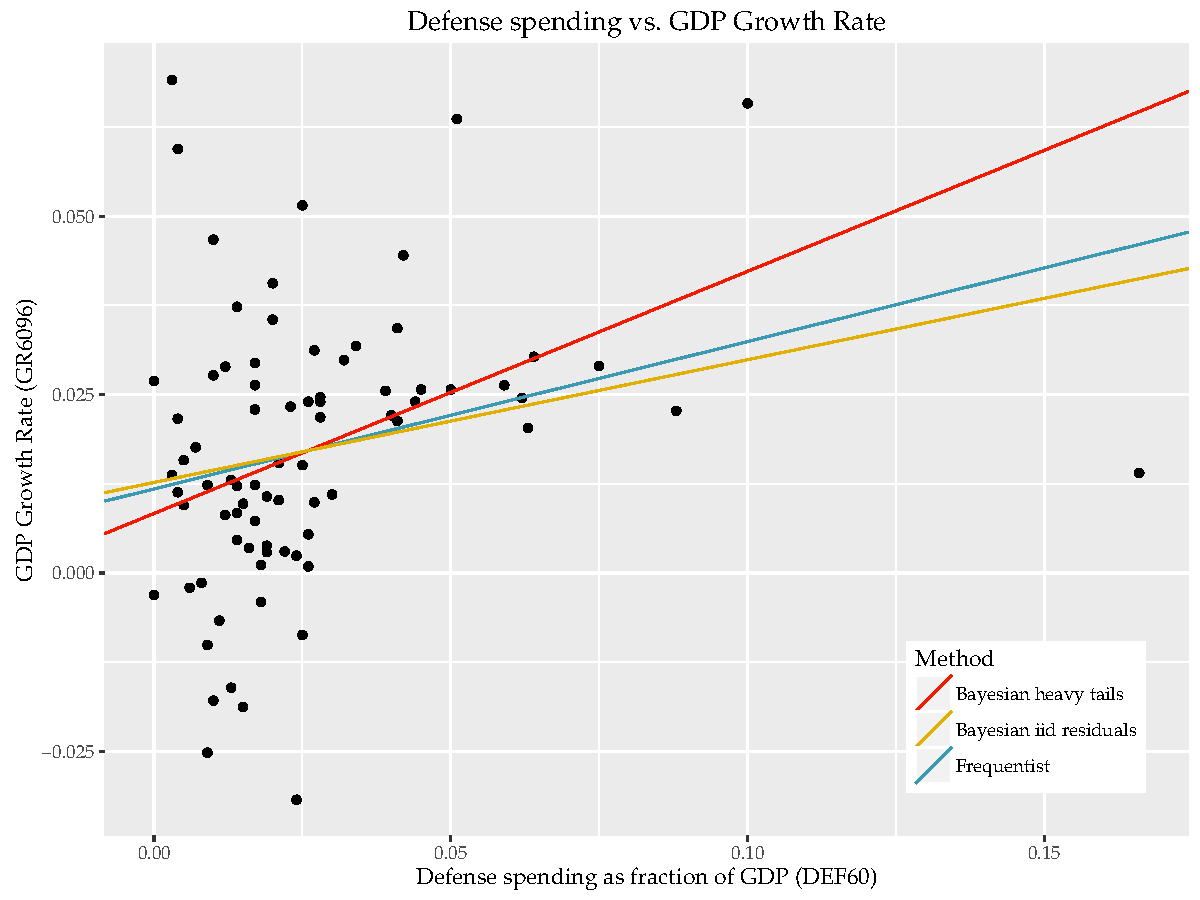
\includegraphics[scale=0.65]{img/compplot.pdf}
		\caption{Comparison of three methods}
		\label{fig:compfig}
	\end{figure}
	%
	%
	%
\end{enumerate}

\end{homeworkProblem}



%%----------------------------------------------------------------------------------------
%%	LIST CODE
%%----------------------------------------------------------------------------------------

\pagebreak
% \rscript{homework03.r}{Sample Perl Script With Highlighting}
R code for \texttt{myfuns02.R}
\lstinputlisting[language=R]{myfuns02.R}
\pagebreak
R code for \texttt{exercises02.R}
\lstinputlisting[language=R]{exercises02.R}


%----------------------------------------------------------------------------------------

\end{document}